\begin{enumerate}
    \item Given point $\vec{P} = \myvec{-4\\3}$ and slope $m = \frac{1}{2}$.
    The direction vector is $\vec{m} = \myvec{2\\1}$.  
    Hence, the normal vector
    \begin{align}
    \label{linform/2/14/eq:line_norm_dir}
    \vec{n} &= \myvec{0&-1\\1&0}\vec{m} 
    \\
    &= \myvec{-1\\2}
    \end{align}
    The equation of the line in terms of the normal vector is then obtained as
    \begin{align}
    \label{linform/2/14/eq:line_norm_vec}
    \vec{n}^T\brak{\vec{x}-\vec{A}} &= 0
    \\
    \implies \myvec{-1 & 2} \vec{x} &= 10
    \end{align}
    See Fig.     \ref{linform/2/14/Plot of Line AB (Part-1)}
    \begin{figure}[ht]
    \centering
    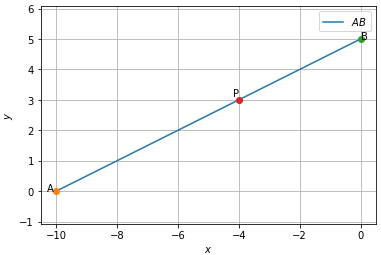
\includegraphics[width=\columnwidth]{solutions/su2021/2/14/Line_Plot_Part1.PNG}
    \caption{Plot of Line $AB$ (Part-1)}
    \label{linform/2/14/Plot of Line AB (Part-1)}
    \end{figure}
    \item Given point $\vec{P} = \myvec{2\\2\sqrt{3}}$.From the given information we have, $\tan75\degree =m = \frac{\sqrt{3}+1}{\sqrt{3}-1}$.
    The direction vector is $\vec{m} = \myvec{1\\\tan75\degree}$.  
    Hence, the normal vector
    \begin{align}
    \label{linform/2/14/eq:line_norm_dir2}
    \vec{n} &= \myvec{0&-1\\1&0}\vec{m} 
    \\
    &= \myvec{-\tan75\degree\\1}
    \end{align}
    The equation of the line in terms of the normal vector is then obtained as
    \begin{align}
    \label{linform/2/14/eq:line_norm_vec2}
    \vec{n}^T\brak{\vec{x}-\vec{A}} &= 0
    \\
    \implies \myvec{-\sqrt{3}+1 &\sqrt{3}-1}  \vec{x} &= -4\brak{\sqrt{3}-1}
    \end{align}
    See Fig. \ref{linform/2/14/Plot of Line AB (Part-2)}

    \begin{figure}[ht]
    \centering
    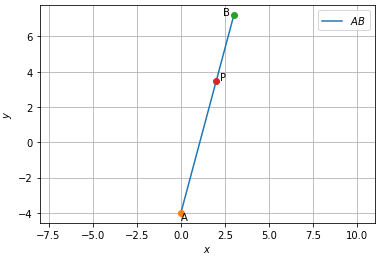
\includegraphics[width=\columnwidth]{solutions/su2021/2/14/Line_Plot_Part2.PNG}
    \caption{Plot of Line $AB$ (Part-2)}
    \label{linform/2/14/Plot of Line AB (Part-2)}
    \end{figure}
